\documentclass[11pt]{article}

\usepackage[margin=1in]{geometry}
\usepackage{amsmath}
\usepackage{graphicx}
\usepackage{booktabs}
\usepackage{caption}
\usepackage{microtype}
\usepackage[T1]{fontenc}
\usepackage{lmodern}
\usepackage[round]{natbib}
\usepackage[hidelinks]{hyperref}

\hypersetup{
  pdftitle={When Routing Entropy Tracks Length, Not Complexity: A Cross-Model Token-Position Confound in MoE Interpretability},
  pdfauthor={Jeffrey Shorthill},
  pdfkeywords={mixture-of-experts, routing entropy, token position, prompt length confound, prefill, interpretability, MoE language models}
}

\captionsetup{font=small,labelfont=bf}
\setlength{\parskip}{0.35em}

\title{\textbf{When Routing Entropy Tracks Length, Not Complexity:\\
A Cross-Model Token-Position Confound in MoE Interpretability}}
\author{Jeffrey Shorthill\thanks{Independent researcher. Correspondence:
\texttt{jws299792@icloud.com}. This is version~1.0 (June~2026),
released under CC~BY~4.0. Data, code, and a claim-by-claim source index
accompany the paper; see the Data and Code Availability statement.}}
\date{Version 1.0 --- June 2026}

\begin{document}
\maketitle

\begin{abstract}
\noindent
Mixture-of-experts (MoE) language models send each token to a small subset of
experts. The entropy of that routing distribution (how evenly a token's weight
spreads across experts) is a convenient one-number summary, and a higher value
invites reading as a sign that the model is working harder. Across a 168-prompt
suite graded into twelve levels of intended cognitive complexity, the routing
entropy averaged over all prefill tokens rises with the intended level in two
MoE models (DeepSeek V3.1, Spearman $\rho = +0.80$; Qwen3.5-397B, $\rho = +0.62$;
$n = 168$ each). The same averaged quantity tracks prompt token count more
strongly ($\rho = +0.88$ and $+0.78$). Routing entropy rises with token position
inside the prefill, so longer prompts, which the complexity grading also makes
longer, collect more high-entropy late positions and lift the all-token mean.
Reading routing entropy at the final prefill token, whose receptive field already
spans the whole prompt, removes the gradient: the correlation with level falls to
$\rho = +0.02$ ($p = 0.82$) for DeepSeek V3.1 and $\rho = -0.06$ ($p = 0.42$) for
Qwen, and a level-1 versus level-12 comparison reverses sign, with the short
prompts showing slightly higher final-token entropy. The reversal holds at
$p < 10^{-3}$ in both models, and the all-token pattern repeats in a DeepSeek R1
run on the same suite. In this setup the aggregate gradient reflects token count
and token position. We describe the readout that removes it, the mechanism behind
the inflation, and the length-matched follow-up that would settle what remains.
\end{abstract}

\noindent\textbf{Keywords:} mixture-of-experts; routing entropy; token position;
prompt-length confound; prefill; interpretability.

\section{Introduction}
\label{sec:intro}

A routing analysis of a mixture-of-experts model starts from a simple object: for
each token, the router produces a distribution over experts and keeps the top few.
Summary statistics of that distribution are easy to compute and easy to compare
across prompts. Routing entropy---the spread of the per-token routing
distribution---is one such statistic. It is appealing as a workload readout because
a peaked distribution looks like confident specialization and a flat distribution
looks like the model hedging across many experts.

This note follows one such reading and reports where it breaks. We graded a prompt
suite into twelve levels meant to span increasing cognitive demand, from rote
repetition up to layered self-referential prompts, and measured routing entropy on
two MoE models. Averaged over the tokens of each prompt, routing entropy climbs
with the intended level. Taken alone, that gradient supports treating the statistic
as a complexity proxy.

The gradient has a second explanation. The graded prompts also grow longer with
level, and the averaged statistic tracks prompt length at least as tightly as it
tracks the grading. The reason is positional: within a single prefill pass, later
token positions carry higher routing entropy on average, because under causal
attention they read a larger context. Averaging entropy over all positions gives
long prompts more weight from their high-entropy tail, so length raises the mean on
its own. Moving the measurement to the final prefill token, a single position whose
receptive field already covers the whole prompt, removes the positional averaging.
Under that readout the gradient with level disappears in both models, and the
extreme levels swap order.

The result is narrow. It concerns one prompt suite, one pair of models, and one way
of aggregating a routing statistic. The point to carry away is mechanical: when
routing entropy is averaged over prompts of different lengths, prompt length can
stand in for whatever the prompts were meant to vary.

The contribution is a measurement caution with a worked diagnosis. We document the
apparent complexity gradient in the all-token mean across two MoE models and a
replication; we show the same statistic tracks prompt token count at least as
tightly; we trace the inflation to a positional effect, that routing entropy rises
with token position within the prefill; and we give a position-controlled readout,
the final prefill token, under which the gradient with intended level disappears
and the extreme levels swap order.

\section{Related work}
\label{sec:related}

\paragraph{Mixture-of-experts routing and its summary statistics.}
A mixture-of-experts layer routes each token through a learned gate to a few of many
expert subnetworks \citep{jacobs1991adaptive,shazeer2017outrageously}, a design
scaled into large transformers by Switch Transformers \citep{fedus2022switch} and,
in the models studied here, by the fine-grained-expert routing of DeepSeek
\citep{dai2024deepseekmoe,deepseekai2024v3,deepseekai2025r1} and the Qwen3 lineage
\citep{yang2025qwen3}. Because the router emits an inspectable distribution at every
token, summary statistics of that distribution are a common readout; routing
analyses of this kind go back at least to the per-token study of Mixtral
\citep{jiang2024mixtral}, and the Shannon entropy of the routing weights is one such
one-number summary.

\paragraph{Routing signals read as difficulty or effort.}
A line of work treats the router's distribution as a difficulty signal.
\citet{huang2024harder} make this explicit, activating more experts for inputs the
router is less confident about, on the premise that harder inputs warrant more
computation; mixture-of-depths \citep{raposo2024mixture} routes a per-token compute
budget on a related premise. Reading a flat (high-entropy) routing distribution as a
sign that the model is working harder is the intuition this note examines. We do not
dispute that the router responds to input; we show that a between-prompt gradient in
\emph{averaged} routing entropy can be produced by prompt length and token position,
so an aggregate gradient is weak evidence on its own that the experts are responding
to intended complexity.

\paragraph{Position-dependent behavior and length confounds.}
Causal self-attention \citep{vaswani2017attention} makes a token's representation
depend on every earlier position, so later positions are computed over more context,
and transformers are known to behave sharply differently across positions, for
instance the attention sinks at initial positions documented by
\citet{xiao2024streaming}. The mechanism we report is in this family: routing
entropy rises with prefill position, so averaging over positions over-weights the
high-entropy tails of long prompts. That length can stand in for an intended factor
is a familiar hazard elsewhere; in reinforcement learning from human feedback, for
example, a length-only proxy reproduces much of an apparent quality gradient
\citep{singhal2024length}. The same hazard appears here for a routing statistic. A
companion analysis by the present author separates the prefill and generation passes
for a different routing question, expert--domain specialization
\citep{shorthill2026generation}; the prefill capture and prefill/generation framing
are shared, the measured quantity is not.

\section{Why routing entropy is tempting as a complexity readout}
\label{sec:tempting}

Three properties make routing entropy attractive as a between-prompt measure.

It is cheap and intrinsic. The router already computes the distribution during a
forward pass, so capturing it adds no probes, no fitted readout, and no labels. A
prefill-only pass over a prompt set yields a number per token at every MoE layer.

It has a clean interpretation per token. Low entropy means the token's weight
concentrates on a few experts; high entropy means it spreads out. Read locally,
that is a statement about how committed the router is at that position, and it is
tempting to extend the local reading to a whole prompt by averaging.

It moves with things researchers care about. In the suite studied here, the
all-token mean rises smoothly across the twelve graded levels in both models
(Figure~\ref{fig:level}, circles). A monotonic climb across a deliberately ordered
factor is the kind of pattern that invites a one-line summary: ``harder prompts
route more diffusely.''

The averaging step is where the reading becomes fragile. A per-token quantity
becomes a per-prompt quantity only after a choice of how to pool positions, and the
mean over all prefill tokens is not neutral with respect to prompt length. The rest
of this note works through that step.

\section{Methods}
\label{sec:methods}

\paragraph{Models.}
We use two mixture-of-experts models. DeepSeek V3.1 \citep{deepseekai2024v3} has
256 experts with 8 active per token across 58 MoE layers;
Qwen3.5-397B-A17B \citep{yang2025qwen3} has 512 experts with 10 active across 60 MoE
layers. Both were run from quantized weights
(\texttt{UD-Q2\_K\_XL}) on a llama.cpp fork (build \texttt{b8123},
\texttt{capture\_activations}), with greedy decoding and routing captured in
prefill-only mode (\texttt{n\_predict} $=0$). A DeepSeek R1 run
\citep{deepseekai2025r1} on the same suite serves as a replication. The router output recorded at each prefill token, for each
MoE layer, is the input to every measurement below.

\paragraph{Prompt suite.}
The suite holds 168 prompts: 14 prompts at each of 12 levels. The levels are an
intended-complexity ordering, from rote repetition and factual recall at the low
end, through logical reasoning, analogy, theory-of-mind, and ethical dilemmas, up to
self-referential and persona-style prompts at the high end. The levels were written
to vary in cognitive demand. They also vary in length: the low levels are short
(mean near 30 tokens) and several high levels run long (the longest level averages
about 150 tokens). That length structure is the confound this note tracks.

\paragraph{Routing entropy.}
At a token, each MoE layer's router yields weights over its experts; we take the
Shannon entropy of that weight distribution, average across the model's MoE layers,
and normalize to the unit interval, giving a per-token routing entropy in
$[0, 1]$. We summarize a prompt two ways. The \emph{all-token mean} averages the
per-token value over every prefill position. The \emph{final-token} readout takes
the value at the last prefill position only. Under causal attention the final
position has attended to the entire prompt, so its routing entropy is a
single-position summary that does not average over the length of the prompt.

\paragraph{Statistics.}
For each model we compute Spearman rank correlations over all $n = 168$ prompts
between routing entropy and (i) the intended level and (ii) the prompt token count,
for both the all-token and final-token readouts. We compare the lowest and highest
levels (L1, $n=14$; L12, $n=14$) with a Wilcoxon rank-sum test. The intended-level
correlation is the quantity a complexity reading would lean on; the token-count
correlation is the confound; the final-token readout is the position-controlled
check.

\section{Results}
\label{sec:results}

\subsection{The all-token mean rises with the intended level}

Averaged over all prefill tokens, routing entropy increases across the twelve
levels in both models (Figure~\ref{fig:level}, circles). The Spearman correlation
with level is $\rho = +0.80$ ($p \approx 5.6\times10^{-39}$) for DeepSeek V3.1 and
$\rho = +0.62$ ($p \approx 5.7\times10^{-19}$) for Qwen
(Table~\ref{tab:spearman}). Read on its own, this is the gradient a complexity
proxy would predict.

\begin{figure}[t]
\centering
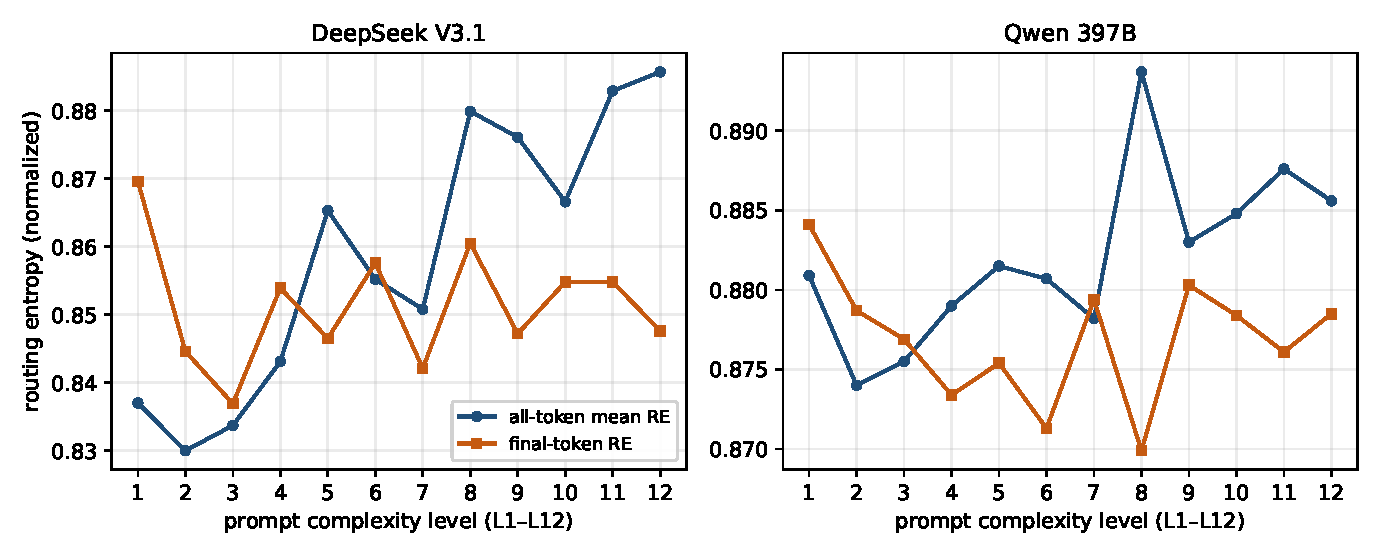
\includegraphics[width=\textwidth]{figures/fig1_level_means.pdf}
\caption{Per-level mean routing entropy against intended complexity level, for
DeepSeek V3.1 (left) and Qwen 397B (right). Circles: all-token mean routing
entropy. Squares: final-token routing entropy. Each point averages 14 prompts;
168 prompts per model. The all-token mean climbs with level in both models; the
final-token readout stays within a narrow band with no monotonic trend.}
\label{fig:level}
\end{figure}

\subsection{The same average tracks token count more strongly}

The graded levels grow longer toward the high end, and the all-token mean follows
length closely. Across all 168 prompts it correlates with token count at
$\rho = +0.88$ ($p \approx 1.8\times10^{-55}$) for DeepSeek V3.1 and $\rho = +0.78$
($p \approx 8.3\times10^{-36}$) for Qwen. In both models the correlation with token
count is tighter than the one with level. Figure~\ref{fig:tokens} shows the per-level means against
per-level mean token count for DeepSeek V3.1: the entropy ordering and the length
ordering largely coincide. Token count and intended level are themselves strongly
related in this suite, so a measure that rises with length will also rise with
level.

\begin{figure}[t]
\centering
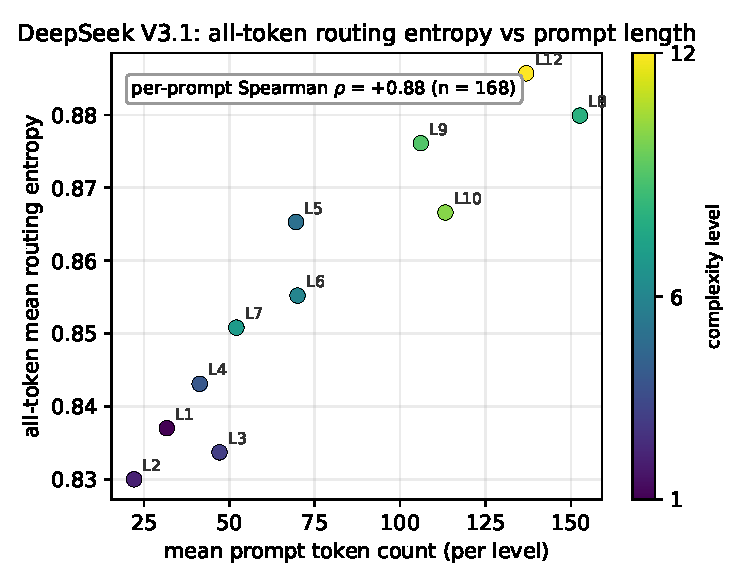
\includegraphics[width=0.62\textwidth]{figures/fig2_token_confound.pdf}
\caption{DeepSeek V3.1 per-level all-token mean routing entropy against per-level
mean prompt token count; markers labeled and colored by level. The annotated
correlation is the per-prompt Spearman value over all 168 prompts. All-token mean
routing entropy and prompt length rise together.}
\label{fig:tokens}
\end{figure}

\subsection{The final-token readout removes the gradient}

Measured at the final prefill token, routing entropy no longer orders by level
(Figure~\ref{fig:level}, squares). The correlation with level falls to
$\rho = +0.02$ ($p = 0.82$) for DeepSeek V3.1 and $\rho = -0.06$ ($p = 0.42$) for
Qwen (Table~\ref{tab:spearman}). The final-token correlation with token count is
also small ($\rho = +0.16$ and $\rho = -0.22$), in line with a single-position
readout that does not pool over length. Figure~\ref{fig:spearman} places the four
correlations side by side: large and positive for the all-token readout, near zero
for the final-token readout, in both models.

\begin{table}[t]
\centering
\caption{Spearman correlations of routing entropy with intended level and with
prompt token count, by readout and model ($n = 168$). The all-token mean orders by
level and by length; the final-token readout does neither.}
\label{tab:spearman}
\small
\begin{tabular}{llrr}
\toprule
Model & Readout & vs.\ level ($\rho$, $p$) & vs.\ token count ($\rho$, $p$) \\
\midrule
DeepSeek V3.1 & all-token  & $+0.80$ \ ($5.6\times10^{-39}$) & $+0.88$ \ ($1.8\times10^{-55}$) \\
DeepSeek V3.1 & final-token & $+0.02$ \ ($0.82$)             & $+0.16$ \ ($0.037$) \\
Qwen 397B     & all-token  & $+0.62$ \ ($5.7\times10^{-19}$) & $+0.78$ \ ($8.3\times10^{-36}$) \\
Qwen 397B     & final-token & $-0.06$ \ ($0.42$)             & $-0.22$ \ ($0.0042$) \\
\bottomrule
\end{tabular}
\end{table}

\begin{figure}[t]
\centering
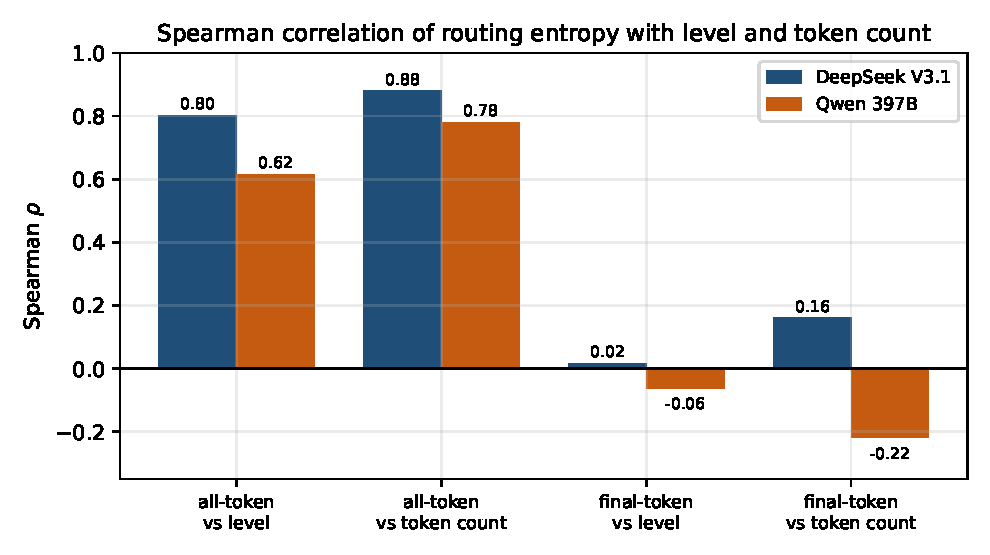
\includegraphics[width=0.82\textwidth]{figures/fig3_spearman.pdf}
\caption{Spearman correlation of routing entropy with intended level and with
prompt token count, for each readout and model ($n = 168$). The two left groups
use the all-token mean; the two right groups use the final-token readout. The
correlation with level is large under all-token aggregation and near zero at the
final token.}
\label{fig:spearman}
\end{figure}

\subsection{The extreme levels swap order}

A direct comparison of the lowest and highest levels shows the same thing as a
direction change. Under the all-token mean, level 12 sits above level 1 in both
models (DeepSeek V3.1, $W = -4.00$, $p = 6.4\times10^{-5}$; Qwen, $W = -2.94$,
$p = 3.3\times10^{-3}$). Under the final-token readout the order flips: level 1
sits above level 12 (DeepSeek V3.1, $W = +3.77$, $p = 1.7\times10^{-4}$; Qwen,
$W = +3.31$, $p = 9.4\times10^{-4}$), shown in Table~\ref{tab:reversal}. At a single
position that already covers the whole prompt, the short, low-level prompts carry
slightly higher routing entropy than the long, high-level ones. The gap is larger
in DeepSeek V3.1 (about 0.022) than in Qwen (about 0.006).

\begin{table}[t]
\centering
\caption{Level-1 versus level-12 routing entropy (Wilcoxon rank-sum, $n=14$ per
level). The all-token mean places the complex level higher; the final-token readout
places the simple level higher.}
\label{tab:reversal}
\small
\begin{tabular}{llrrl}
\toprule
Model & Readout & L1 mean & L12 mean & Direction ($p$) \\
\midrule
DeepSeek V3.1 & all-token   & 0.837 & 0.886 & L12 $>$ L1 \ ($6.4\times10^{-5}$) \\
DeepSeek V3.1 & final-token & 0.870 & 0.848 & L1 $>$ L12 \ ($1.7\times10^{-4}$) \\
Qwen 397B     & all-token   & 0.881 & 0.886 & L12 $>$ L1 \ ($3.3\times10^{-3}$) \\
Qwen 397B     & final-token & 0.884 & 0.879 & L1 $>$ L12 \ ($9.4\times10^{-4}$) \\
\bottomrule
\end{tabular}
\end{table}

\subsection{The pattern is consistent across runs}

A DeepSeek R1 run on the same 168-prompt suite reproduces the all-token picture:
routing entropy correlates with level at $\rho = +0.84$ and with token count at
$\rho = +0.86$, again ordering by length at least as well as by level. The earlier
98-prompt baseline on DeepSeek V3.1 showed the same signature on the generation
side, where the all-token mean correlated with generated length ($\rho = +0.51$,
$p \approx 5\times10^{-7}$) more clearly than with level ($\rho = +0.20$,
$p = 0.05$). The positional dependence behind these patterns was checked directly
with a per-token diagnostic, in which routing entropy rises with token position
within the prefill.

A separate, tightly templated prompt suite gives a preliminary cross-check in the
other direction. From a forced-choice triage set with uniform scaffolding and a
narrow length band (227--245 tokens), only 17 of 32 prompts survived as raw
captures, all in the three lowest levels. On that subset the all-token mean
correlates negatively with both token count ($\rho = -0.66$) and level
($\rho = -0.58$), and token count again accounts for more of the variance than
level. Because the subset is small and spans only three levels, we treat it as a
preliminary note that the readout stays sensitive to prompt construction, not as a
second gradient.

\section{Interpretation}
\label{sec:interp}

\paragraph{Why averaging over positions favors long prompts.}
Under causal attention \citep{vaswani2017attention}, the representation at a prefill
position depends on every earlier position, so later tokens are computed over more
context. In both models
the router responds to that by spreading weight a little more widely at later
positions, which raises per-token routing entropy with position. The all-token mean
weights every position equally, so it collects more high-entropy positions from a
long prompt than from a short one. When the prompt set is ordered so that the
intended-complexity levels also grow longer, the mean rises with level on length
alone. The final-token readout avoids the pooling step: it reports one position
whose context is the full prompt, so every prompt contributes a single value
regardless of length.

\paragraph{The reversal.}
At the final token, the short low-level prompts carry slightly higher routing
entropy than the long high-level prompts, and the difference is consistent across
both models. A plain reading is that with less prior context to condition on, the
router at the final position spreads weight a little more widely. We offer that as a
description of the measured direction; the mechanism stays open. The effect is small
(about 0.02 and 0.006 in normalized entropy), and a stronger account would need a
position-resolved analysis.

\paragraph{Scope of the claim.}
What these runs support is specific. In this suite and these two models, the
all-token mean routing entropy orders prompts by length and by token position, and
a position-controlled readout does not reproduce the ordering by intended
complexity. The finding speaks to one way of turning a per-token routing statistic
into a per-prompt number when prompts differ in length. It does not establish that
routing entropy carries no information about prompt content, and it does not bear on
routing analyses that hold length fixed or that model position explicitly.

\section{Limitations and falsification tests}
\label{sec:limits}

\paragraph{Limitations.}
The intended-complexity grading and prompt length are entangled in this suite, so
these runs separate position from the all-token average but do not yet separate
length from complexity; a length-matched suite is the missing control. The
final-token readout removes the positional averaging at the cost of resting on a
single position, which carries its own sampling noise. The proposed reason for the
final-token reversal is a description of direction, not a demonstrated mechanism.
The evidence covers two model families plus an R1 replication, all from quantized
weights under one inference setup; other architectures and precisions are untested
here. The result diagnoses one measurement setup; an all-token average stays useful
when position and length are modeled directly.

\paragraph{Tests that would weaken or overturn this reading.}
The following are proposed, not yet run.
\begin{itemize}\setlength{\itemsep}{0.2em}
\item \textbf{Length-matched complexity prompts.} Hold token count fixed across
levels. If the all-token gradient with level survives at matched length, the
token-count explanation weakens.
\item \textbf{Fixed-token-budget variants.} Pad or trim prompts to a common budget
and re-measure both readouts.
\item \textbf{Within-position entropy curves by level.} Compare entropy-versus-position
curves across levels; overlapping curves would attribute the all-token gap to
position, separated curves would not.
\item \textbf{Final-token plus mean-of-last-$k$.} Compare the single final position
with an average over the last $k$ positions to gauge single-position noise against
the positional control.
\item \textbf{More MoE families.} Repeat on additional architectures and precisions
to test whether the positional dependence is general.
\item \textbf{Token-count-preserving paraphrase.} Shuffle or paraphrase prompts
within a level while holding token count, to separate wording from length.
\item \textbf{Mixed-effects regression.} Model routing entropy with token count,
position, model, and level together, and ask whether level retains an effect once
the first three are included.
\end{itemize}

\section{Conclusion}
\label{sec:conc}

In this setup, aggregate routing entropy tracks token count and token position. The
twelve-level gradient that looked like a complexity signal under the all-token mean
follows prompt length at least as closely, and it comes apart at the final prefill
token, where the ordering by level disappears and the extreme levels change places.
The same all-token signature appears across DeepSeek V3.1, a DeepSeek R1
replication, and Qwen 397B. The practical takeaway is concrete: when
routing entropy is compared across prompts of different lengths, report it at a
position-controlled readout, or model position and length directly, before reading
a between-prompt difference as a difference in what the prompts demand. A
length-matched suite would settle how much, if any, of the level effect remains once
length is held fixed.

\section*{Reproducibility and audit note}

The measurements above are recomputed in this paper's \texttt{make\_figures.py} from
files in a preserved archive (\texttt{token-confound-archive/}). The per-level means
and summary correlations are transcribed from the archive's evidence summary
(\texttt{CROSS\_MODEL\_POSITION\_CONFOUND.md}), which matches the project journal's
record of the same run. Per-level token counts are computed from the DeepSeek V3.1
per-prompt summary (\texttt{data/ds31-168q-1\_prefill.json}); the DeepSeek R1
per-prompt routing entropy and token counts are read from
\texttt{raw/\allowbreak 168q-r1-deepseek-r1/\allowbreak results\_\allowbreak 168\_\allowbreak r1\_\allowbreak prefill.json}.
The per-token
position diagnostic is in \texttt{data/diagnostic\_results.json}. A source-to-claim
index is given in \texttt{SOURCES.md}.

The archive keeps the trail that led here. An earlier generation-phase measurement
on a 30-turn run reported a sharp peak on the final turn; that turn was also the
longest generation, and the peak was set aside once length was recognized as its
driver---the same length sensitivity that this note isolates on the prefill side.
The archive also records a data-integrity event from that period: while assembling
result tables, an automated step produced per-prompt rows that matched the correct
aggregates but were not extracted from the run logs, and some per-prompt slope signs
were wrong as a result. The tables were regenerated from the logs and a
verify-against-log rule was added. The aggregate correlations reported in this paper
are the verified, log-derived values, and the earlier per-prompt write-ups that
predate the position control are retained in the archive as superseded.

\section*{Data and Code Availability}
\addcontentsline{toc}{section}{Data and Code Availability}

The measurements in this paper are recomputed from a preserved capture archive
(\texttt{token-confound-archive/}) by \texttt{make\_figures.py}, which fits the three
figures and the reported correlations from the per-prompt routing-entropy and
token-count records and re-runs no model. The per-level summaries and correlations
are transcribed from the archive's evidence summary
(\texttt{CROSS\_MODEL\_POSITION\_CONFOUND.md}); per-prompt token counts and the
DeepSeek R1 replication values are recomputed from the archived per-prompt JSON, and
the per-token position diagnostic from \texttt{data/diagnostic\_results.json}. A
claim-by-claim source index is given in \texttt{SOURCES.md}. No new model training
was performed.

\section*{AI Collaboration Statement}
\addcontentsline{toc}{section}{AI Collaboration Statement}

Generative AI (Anthropic's Claude) was used as a tool in preparing this manuscript:
to assist with drafting and revising prose, organizing the manuscript, and locating
and formatting the bibliography. All captures, statistics, and numerical results are
the author's; every reported value was traced to a source capture (see
\texttt{SOURCES.md}), and every reference was verified by the author against its
authoritative record to exist and to support the statement it is attached to. No AI
system is an author. The author reviewed the entire text and takes full
responsibility for its content, including any errors.

\section*{Funding and Competing Interests}
\addcontentsline{toc}{section}{Funding and Competing Interests}

This work received no external funding. The author declares no competing interests.
The models studied are third-party releases used as-is for measurement; the author
has no affiliation with their creators.

\bibliographystyle{plainnat}
\bibliography{refs}

\end{document}
